\documentclass[14pt,a4paper]{report}  %紙張設定
\usepackage{xeCJK}%中文字體模組
%\setCJKmainfont{標楷體} %設定中文字體
\setCJKmainfont{MoeStandardKai.ttf}
%\newfontfamily\sectionef{Times New Roman}%設定英文字體
\newfontfamily\sectionef{Nimbus Roman}
\usepackage{enumerate}
\usepackage{amsmath,amssymb}%數學公式、符號
\usepackage{amsfonts} %數學簍空的英文字
\usepackage{graphicx, subfigure}%圖形
\usepackage{fontawesome5} %引用icon
\usepackage{type1cm} %調整字體絕對大小
\usepackage{textpos} %設定文字絕對位置
\usepackage[top=2.5truecm,bottom=2.5truecm,
left=3truecm,right=2.5truecm]{geometry}
\usepackage{titlesec} %目錄標題設定模組
\usepackage{titletoc} %目錄內容設定模組
\usepackage{textcomp} %表格設定模組
\usepackage{multirow} %合併行
%\usepackage{multicol} %合併欄
\usepackage{CJK} %中文模組
\usepackage{CJKnumb} %中文數字模組
\usepackage{wallpaper} %浮水印
\usepackage{listings} %引用程式碼
\usepackage{hyperref} %引用url連結
\usepackage{setspace}
\usepackage{lscape}%設定橫式
\lstset{language=Python, %設定語言
		basicstyle=\fontsize{10pt}{2pt}\selectfont, %設定程式內文字體大小
		frame=lines,	%設定程式框架為線
}
%\usepackage{subcaption}%副圖標
\graphicspath{{./../images/}} %圖片預設讀取路徑
\usepackage{indentfirst} %設定開頭縮排模組
\renewcommand{\figurename}{\Large 圖.} %更改圖片標題名稱
\renewcommand{\tablename}{\Large 表.}
\renewcommand{\lstlistingname}{\Large 程式.} %設定程式標示名稱
\hoffset=-5mm %調整左右邊界
\voffset=-8mm %調整上下邊界
\setlength{\parindent}{3em}%設定首行行距縮排
\usepackage{appendix} %附錄
\usepackage{diagbox}%引用表格
\usepackage{multirow}%表格置中
%\usepackage{number line}
%=------------------更改標題內容----------------------=%
\titleformat{\chapter}[hang]{\center\sectionef\fontsize{20pt}{1pt}\bfseries}{\LARGE 第\CJKnumber{\thechapter}章}{1em}{}[]
\titleformat{\section}[hang]{\sectionef\fontsize{18pt}{2.5pt}\bfseries}{{\thesection}}{0.5em}{}[]
\titleformat{\subsection}[hang]{\sectionef\fontsize{18pt}{2.5pt}\bfseries}{{\thesubsection}}{1em}{}[]
%=------------------更改目錄內容-----------------------=%
\titlecontents{chapter}[11mm]{}{\sectionef\fontsize{18pt}{2.5pt}\bfseries\makebox[3.5em][l]
{第\CJKnumber{\thecontentslabel}章}}{}{\titlerule*[0.7pc]{.}\contentspage}
\titlecontents{section}[18mm]{}{\sectionef\LARGE\makebox[1.5em][l]
{\thecontentslabel}}{}{\titlerule*[0.7pc]{.}\contentspage}
\titlecontents{subsection}[4em]{}{\sectionef\Large\makebox[2.5em][l]{{\thecontentslabel}}}{}{\titlerule*[0.7pc]{.}\contentspage}
%=----------------------章節間距----------------------=%
\titlespacing*{\chapter} {0pt}{0pt}{18pt}
\titlespacing*{\section} {0pt}{12pt}{6pt}
\titlespacing*{\subsection} {0pt}{6pt}{6pt}
%=----------------------標題-------------------------=%             
\begin{document} %文件
\sectionef %設定英文字體啟用
\vspace{12em}
\begin{titlepage}%開頭
\begin{center}   %標題  
\makebox[1.5\width][s] %[s] 代表 Stretch the interword space in text across the entire width
{\fontsize{24pt}{2.5pt}國立虎尾科技大學}\\[18pt]
\makebox[1.5\width][s]
{\fontsize{24pt}{2.5pt}機械設計工程系}\\[18pt]
\sectionef\fontsize{24pt}{1em}\selectfont\textbf
{
\vspace{0.5em}
cd2023 2a3-pj3ag1分組報告}\\[18pt]
%設定文字盒子 [方框寬度的1.5倍寬][對其方式為文字平均分分布於方框中]\\距離下方18pt
\vspace{1em} %下移
\fontsize{30pt}{1pt}\selectfont\textbf{網際足球對戰場景設計}\\
\vspace{1em}
\sectionef\fontsize{30pt}{1em}\selectfont\textbf
{
\vspace{0.5em}
Web-based Foosball Scene Design}
 \vspace{2em}
%=---------------------參與人員-----------------------=%             
\end{center}
\begin{flushleft}
\begin{LARGE}

\hspace{32mm}\makebox[5cm][s]
{指導教授:\quad 嚴\quad 家\quad 銘\quad 老\quad 師}\\[6pt]
\hspace{32mm}\makebox[5cm][s]
{班\qquad 級:\quad 四\quad 設\quad 二\quad 甲}\\[6pt]
\hspace{32mm}\makebox[5cm][s]
{學\qquad 生:\quad 王\quad 樟 \quad 皓\quad(41023114)}
\\[6pt]
\hspace{32mm}\makebox[5cm][s]
{\hspace{36.5mm}吳\quad 政 \quad 憲\quad(41023118)}\\[6pt]
\hspace{32mm}\makebox[5cm][s]
{\hspace{36.5mm}呂\quad 承 \quad 劼\quad(41023119)組長}\\[6pt]
\hspace{32mm}\makebox[5cm][s]
{\hspace{36.5mm}呂\quad 昕 \quad 叡\quad(41023120)}\\[6pt]
\hspace{32mm}\makebox[5cm][s]
{\hspace{36.5mm}李\quad 彥 \quad 廷\quad(41023122)}\\[6pt]
\hspace{32mm}\makebox[5cm][s]
{\hspace{36.5mm}李\quad 茂 \quad 廷\quad(41023124)}\\[6pt]
\hspace{32mm}\makebox[5cm][s]
{\hspace{36.5mm}卓\quad 桓 \quad 琮\quad(41023126)}\\[6pt]
\hspace{32mm}\makebox[5cm][s]
{\hspace{36.5mm}林\quad 敬 \quad 燐\quad(41023138)}\\[6pt]
\end{LARGE}
\end{flushleft}
\vspace{6em}
\fontsize{18pt}{2pt}\selectfont\centerline{\makebox[\width][s]
{中華民國\hspace{3em} 
112 \quad 年\quad 6\quad 月}}
\end{titlepage}

%=------------------------摘要-----------------------=%
%\renewcommand{\baselinestretch}{1.5} %設定行距
\pagenumbering{roman} %設定頁數為羅馬數字
\clearpage  %設定頁數開始編譯
\sectionef
\addcontentsline{toc}{chapter}{摘~~~要} %將摘要加入目錄
\begin{center}
\LARGE\textbf{摘~~要}\\
\end{center}
\begin{flushleft}
\fontsize{14pt}{20pt}\sectionef\hspace{12pt}\quad 本課程將採兩人一組、四人一組與八人一組的方式進行協同機電整合產品開發,開發一款能在 web-based CoppeliaSim 場景中雙方或多方 (human or computer) 對玩的遊戲 (game) 產品。最後在 w16 現場發表八人協同四週後所完成的產品,在 w17 各組採 OBS + Teams 以影片發表所完成的協同產品。\\[12pt]

\end{flushleft}
\begin{center}
\fontsize{14pt}{20pt}\sectionef\hspace{12pt}\quad 課程一開始讓學員可以從 https://mde.tw/cd2023/content/BubbleRob.html 導引練習中,了解 CoppeliaSim 套件中的諸多功能以及用法,其中包括利用近接感測器偵測障礙物,並透過 Lua script 控制 bubbleRob 雙輪車的移動。為了讓各組學員了解在多人協同模式下,開發機電資產品流程中必須面臨的許多議題(若要直接在瀏覽器中建立多方協同的場景,可以透過 remote API(導引) 與 Visualization Stream 功能)。再接續專案一的雙輪車,改用 Python zmqRemoteAPI 進行控制,各分組需完成能在 Visualization Stream 瀏覽器中,跨網路雙方各控制一台雙輪車在足球場中進行對陣,且需設計一組能在雙方瀏覽器中進行計分的系統。最後各組需對雙輪車進行設計改良,以提升行進與對戰效能,各組需採 CAD 進行場景與多輪車零組件設計後,轉入足球場景中以鍵盤 arrow keys 與 wzas 等按鍵進行控制,對陣雙方每組將有四名輪車球員,且每兩人在同一台電腦上操作,完成後各組需在分組網站中提供所有相關檔案下載連結,且提供線上分組簡報與分組 pdf 報告連結。\\[12pt]

\end{flushleft}
\begin{center}
\fontsize{14pt}{20pt}\sectionef\hspace{12pt}\quad 專案場景必須要有感測器及記分板,讓進球後可以顯示分數在場景上,而記分板除了採用 LED 顯示計分外,也要以建立以機械轉盤傳動計分系統。另外建立計時器讓學員在對戰時得知時間剩多少,並利用程式控制球門使球重置後繼續對戰,最後在
CoppeliaSim 模擬環境中透過埠號及 http://[2001:288:6004:17:2023:cda:x:x]:23020/ 進行對戰及觀看。\\[12pt]
\newpage
%=--------------------Abstract----------------------=%
\renewcommand{\baselinestretch}{1.5} %設定行距
\addcontentsline{toc}{chapter}{Abstract} %將摘要加入目錄
\begin{center}
\LARGE\textbf\sectionef{Abstract}\\
\begin{flushleft}
\fontsize{14pt}{16pt}\sectionef\hspace{12pt}\quad This course will involve collaborative development of mechatronic integrated products in teams of two, four, and eight members. The objective is to create a web-based game product using CoppeliaSim, where two or more participants (humans or computers) can engage in gameplay within the virtual environment. At the end of the course, during week 16, the eight-member teams will present their completed products in a live demonstration. In week 17, each group will use OBS + Teams to present a video showcasing their collaborative product.\\[12pt]

\end{flushleft}
\begin{center}
\fontsize{14pt}{16pt}\sectionef\hspace{12pt}\quad At the beginning of the course, participants will be guided to practice and explore various functionalities and usage of the CoppeliaSim package through the link https://mde.tw/cd2023/content/BubbleRob.html. This includes using proximity sensors to detect obstacles and controlling the movement of the BubbleRob differential-drive robot using Lua script. In order to familiarize the teams with the challenges encountered in the development of mechatronic products in a multi-user collaborative mode, they will utilize the remote API (guided) and Visualization Stream feature to create a collaborative scenario directly in the web browser. Continuing from Project 1, the teams will switch to using Python zmqRemoteAPI for control. Each group will be required to establish a scenario where two BubbleRob robots, controlled by two separate users over the network, engage in a soccer match within the visualization stream browser. Additionally, the teams need to design a scoring system that can be accessed and displayed in the browsers of both users. In the final stage, each group will improve the design of their BubbleRob robot to enhance its movement and performance during the match. The groups will employ CAD software to design the scene and components of the robots. The control will be switched to using arrow keys and "wzas" keys on the keyboard to maneuver the robots within the soccer field. Each group will have four robot players, with each pair of participants operating on the same computer. Once completed, the groups are required to provide download links for all relevant files on the group website, along with links to online group presentations and PDF reports.\\[12pt]

\end{flushleft}
\begin{center}
\fontsize{14pt}{16pt}\sectionef\hspace{12pt}\quad 
The project scenario requires the presence of sensors and a scoreboard in the simulation environment. The scoreboard should display the score on the scene, indicating goals scored. Apart from using LED displays to show the score, a mechanical rotary-driven scoring system should also be implemented. Additionally, a timer needs to be created to inform the participants about the remaining time during the gameplay. The program should control the goal posts to reset the ball and continue the game. Finally, the participants can engage in the match and observe it through the CoppeliaSim simulation environment using the port address http://[2001:288:6004:17:2023:cda:x:x]:23020/. (Note: Please replace "x" in the provided address with the appropriate values or specific information.)\\[12pt]
\newpage
%=------------------------目錄----------------------=%
\renewcommand{\contentsname}{\centerline{\fontsize{18pt}{\baselineskip}\selectfont\textbf{目\quad 錄}}}
\tableofcontents  %目錄產生
\newpage
%=------------------圖表目錄產生----------------------=%
\renewcommand{\listfigurename}{\centerline{\fontsize{18pt}{\baselineskip}\selectfont\textbf{圖\quad 目\quad 錄 }}}
\newcommand{\loflabel}{圖} %定義\loflabel 文字為圖
\renewcommand{\numberline}[1]{\loflabel~#1\hspace*{0.5em}}
\listoffigures
%\newcommand{\captioname}{圖}
%\end{center}
%=-------------------------內容----------------------=%
\chapter{前言}
\renewcommand{\baselinestretch}{10.0} %設定行距
\pagenumbering{arabic} %設定頁號阿拉伯數字
\setcounter{page}{1}  %設定頁數
\fontsize{14pt}{2.5pt}\sectionef
\section{專案概述與目標}
本課程專案目標需要有場景與多輪車零組件設計、控制程式、開會紀錄與逐字稿、各組員任務分配與執行過程影片及分組報告 pdf 檔案,最後在 w16 現場發表八人協同四週後所完成的產品,在 w17 各組採 OBS + Teams 以影片發表所完成的協同產品。
\begin{figure}[hbt!]
\begin{center}
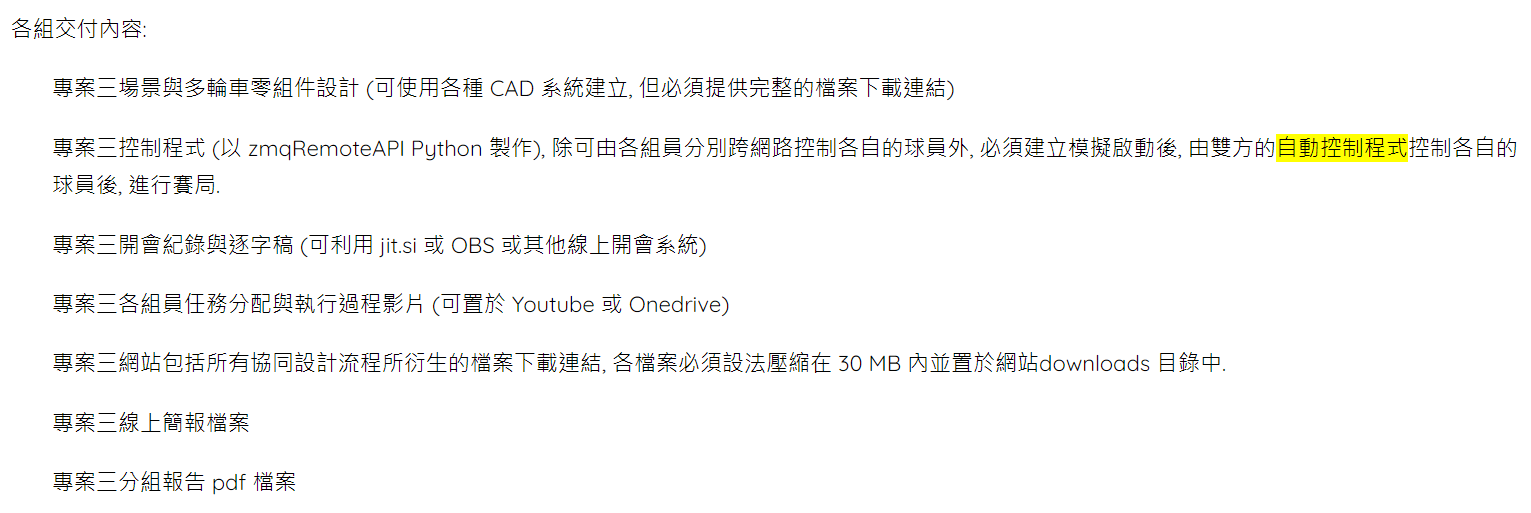
\includegraphics[height=5cm]{work}
\caption{\Large 專案目標}\label{專案目標}
\end{center}
\end{figure} 
\section{規則}
本專題設計理想為一款足球遊戲,比賽一開始球會置於場中央,遊戲開始後雙方即
可鍵盤操控機器人,透過隊友間的傳球並將球送至球門即可得分。\\
遊戲規則如下:\\
球送至敵方球門即得一分。\\
時間內進球數多的一方獲勝。\\
球進入球框後會回到原位。\\
球出界後會回到原位。\\
\renewcommand{\baselinestretch}{0.5} %設定行距
\chapter{討論與分工}
\renewcommand{\baselinestretch}{10.0} %設定行距
\pagenumbering{arabic} %設定頁號阿拉伯數字
\setcounter{page}{24}  %設定頁數
\fontsize{14pt}{2.5pt}\sectionef
\section{分工}

分配工作\\
1.場地設置 41023118 41023138\\
2.車子設計與組裝 41023122 41023124\\
3.輪盤記分板繪製 41023126 41023114\\
4.輪盤記分板程式 41023119 41023120\\
5.車子控制程式與設置 41023119 41023120\\
6.會議記錄 41023126\\
7.整體組合 41023119 41023120\\

\section{討論紀錄}

5/18 會議內容:分配工作\\
1. 場地設置:41023118 41023138\\
2. 車子設計與組裝:41023122 41023124\\
3. 輪盤記分板繪製:41023126 41023114\\
4. 輪盤記分板程式:41023119 41023120\\
5. 車子控制程式與設置:41023119 41023120\\

5/22 會議內容:討論分工的作業情況及尚未完成的事項\\
41023124:車子設計大略完成 剩下背號\\
41023120:程式研究中\\
41023118:場地大致完成 剩下球場線條\\
41023119:機械式記分板程式正在編寫中 球員程式正在編寫中\\
41023126:機械記分板 改第二版\\
41023138:場地大致完成 剩下球場線條\\
41023122:球員除錯\\
41023114:機械記分板外觀研究\\

5/29 會議內容:討論作業情況及模擬場景連線\\
41023122:車子剩下背號\\
41023119:球員程式正在修改中\\
41023138:場景完成\\
和組長做模擬場景連線\\

6/5 會議內容:討論作業情況及latax報告\\
41023119:報告pdf未完成 報告latex摘要完成\\
41023138:正在製作latex報告\\
41023126:繪製機械式計時器cad圖\\
41023124:負責latex第六章 防火牆與ipv6內容設定\\
41023114:負責latex第六章 防火牆與ipv6內容設定\\
\newpage

\renewcommand{\baselinestretch}{1.0} %設定行距
\chapter{場景建立}
\renewcommand{\baselinestretch}{10.0} %設定行距
\pagenumbering{arabic} %設定頁號阿拉伯數字
\setcounter{page}{1}  %設定頁數
\fontsize{14pt}{2.5pt}\sectionef
\section{前言}
老師有規定球場及球員的大小,重量\\
足球規格 (ball): 白色, 直徑 0.1m, 重量 0.5kg\\
足球場地 (field): 長 4m x 寬 2.5m\\
球門規格 (goal[0] and goal[1]: 長 0.6m, 高 0.3m, 寬 0.1m\\
球員尺寸範圍(player[0]-player[7]: 長寬高各 0.2m, 重量 5kg。\\
\section{建立球員}
我們使用CoppeliaSim來製作車子。\\
\

\begin{figure}[hbt!]
\begin{center}
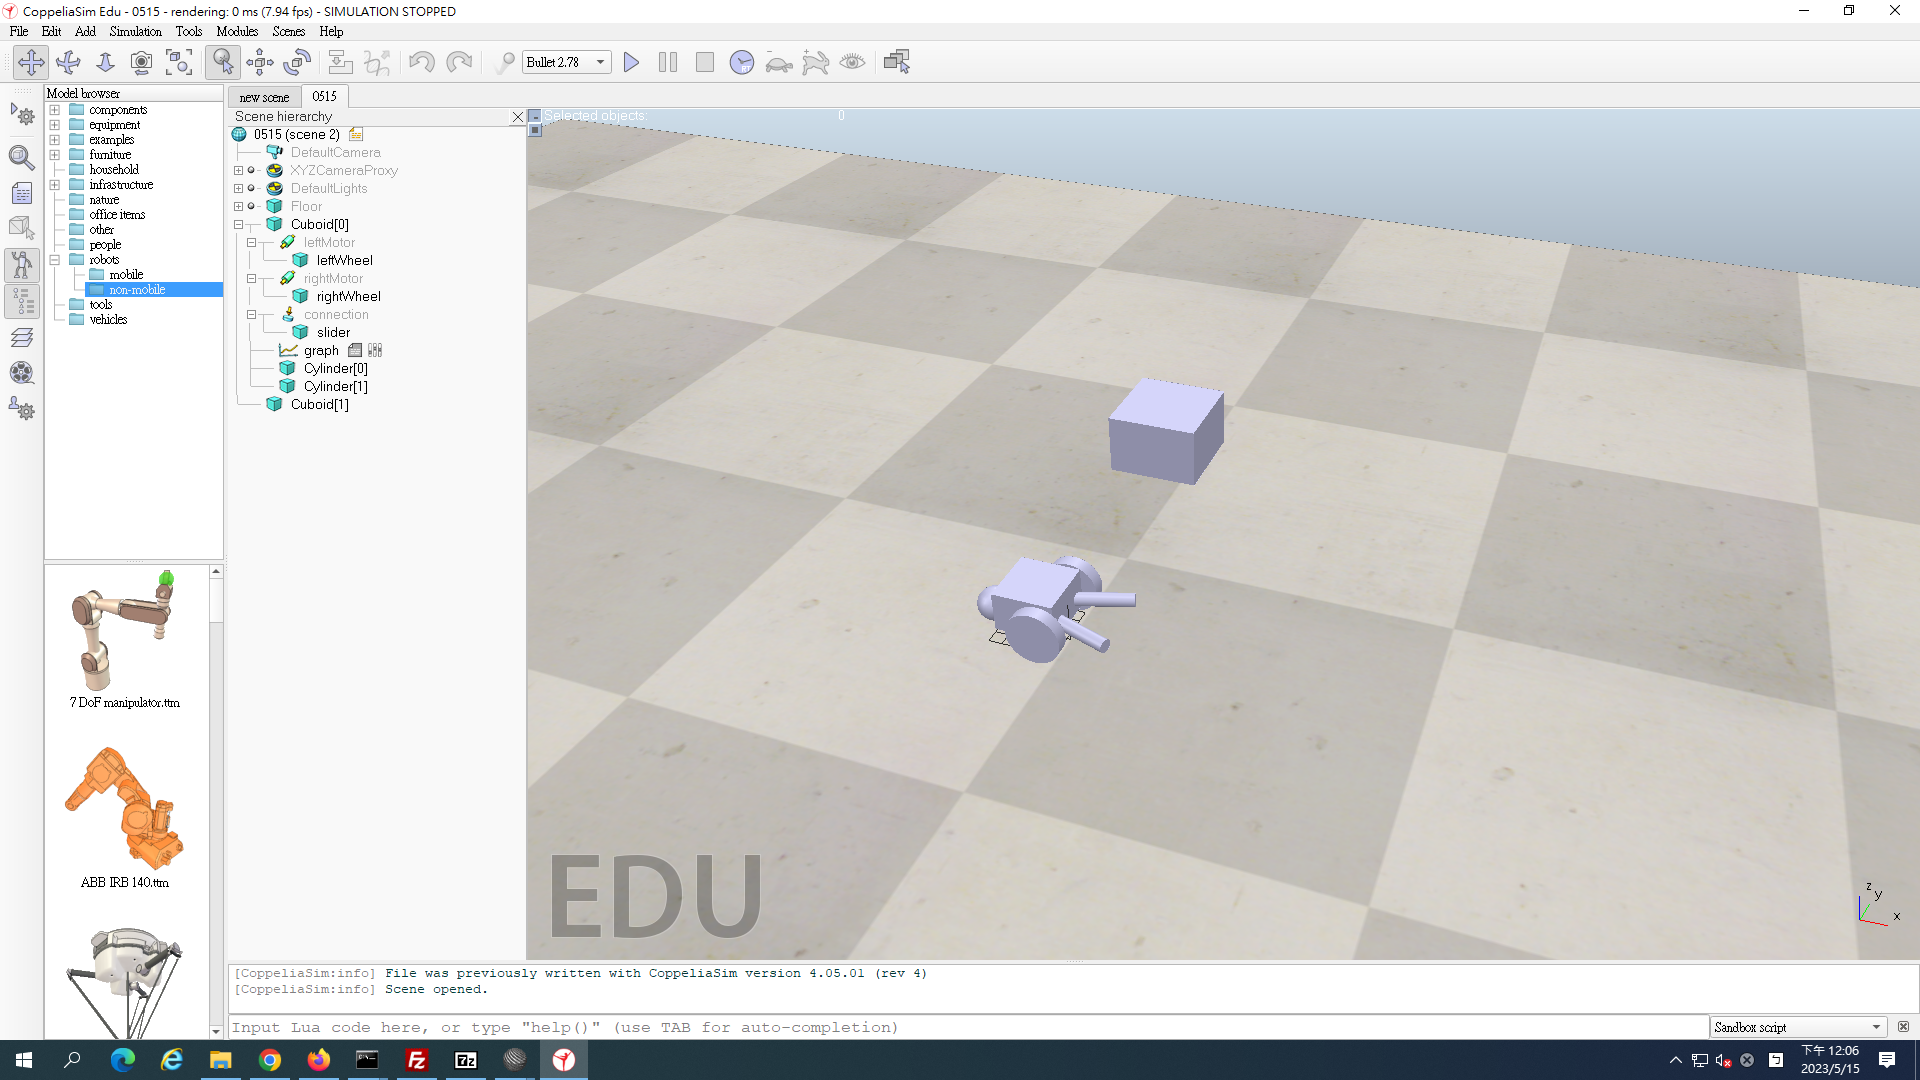
\includegraphics[width=10cm]{0515}
\caption{\Large 球員建立}\label{球員建立}
\end{center}
\end{figure}
\\
\
後發現在移動左右轉彎時會分解,因此直接在CoppeliaSim內修改了定位,且在後背加上號碼。如(圖.\ref{球員建立2})\\

\begin{figure}[hbt!]
\begin{center}
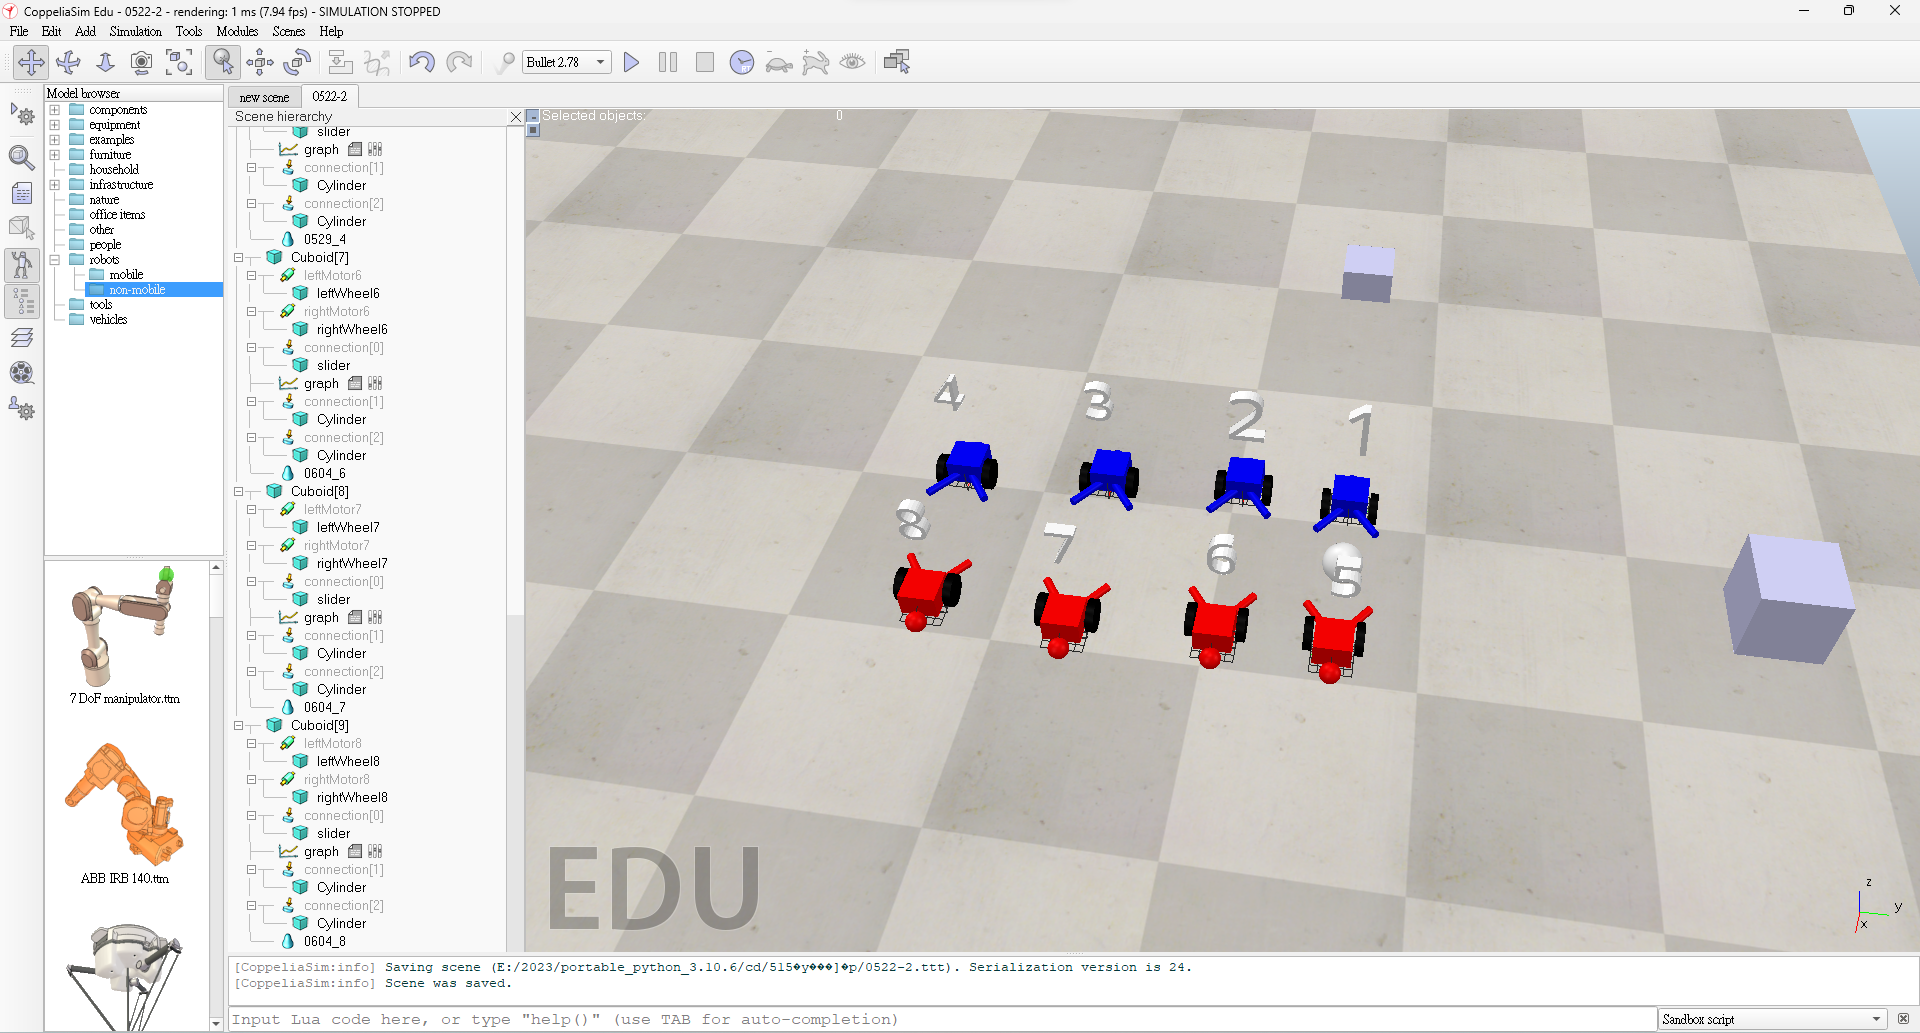
\includegraphics[width=10cm]{0604-1}
\caption{\Large 球員建立2}\label{球員建立2}
\end{center}
\end{figure}\

\section{建立記分板}
我們使用Onshape重新繪製了機械式記分板,如(圖.\ref{記分板建立})\\

\begin{figure}[hbt!]
\begin{center}
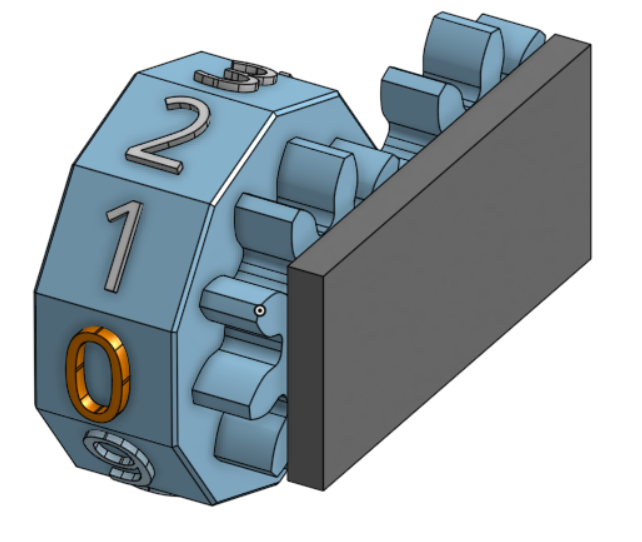
\includegraphics[width=10cm]{輪盤記分板-4-10teeth}
\caption{\Large 記分板建立}\label{記分板建立}
\end{center}
\end{figure}\

\begin{figure}[hbt!]
\begin{center}
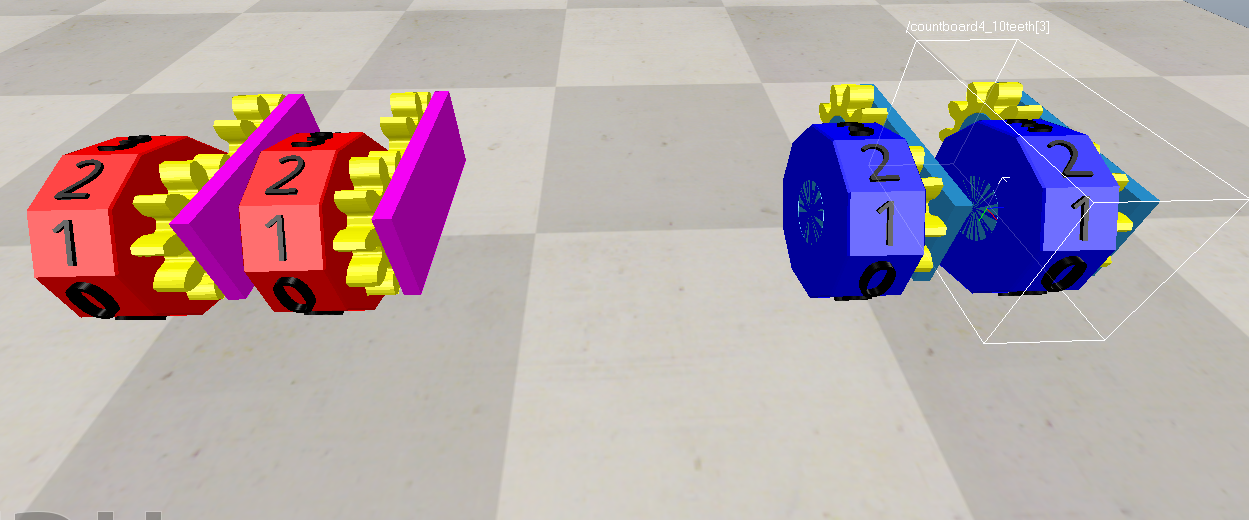
\includegraphics[width=10cm]{Screenshot 2023-05-29 113148.png4-10}
\caption{\Large 匯入記分板}\label{匯入記分板}
\end{center}
\end{figure}\
\newpage
\section{建立球場}
我們使用Onshape繪製了球場底板及球門,如(圖.\ref{球場繪製}),匯入CoppeliaSim後接著建立感測器,如(圖.\ref{建立球場})。\

\begin{figure}[hbt!]
\begin{center}
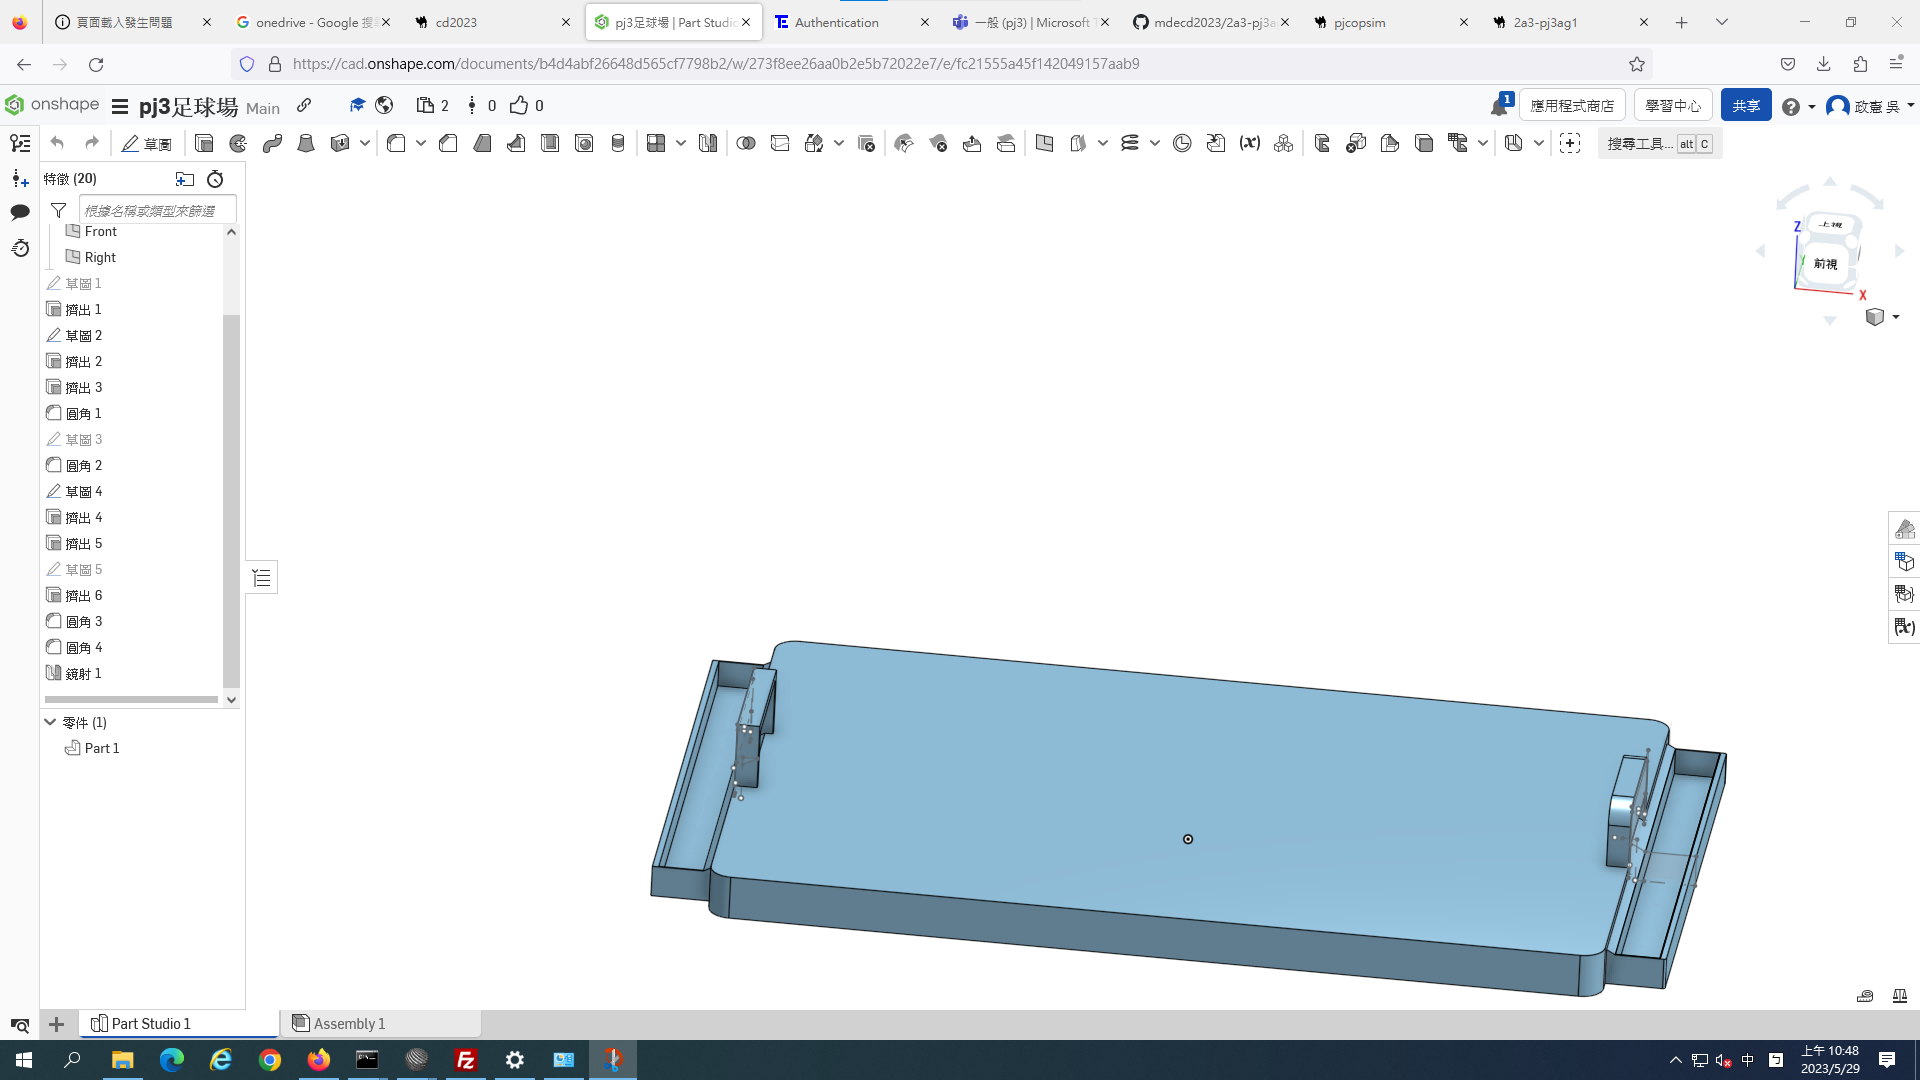
\includegraphics[width=8cm]{33333}
\caption{\Large 球場繪製}\label{球場繪製}
\end{center}
\end{figure}\


\begin{figure}[hbt!]
\begin{center}
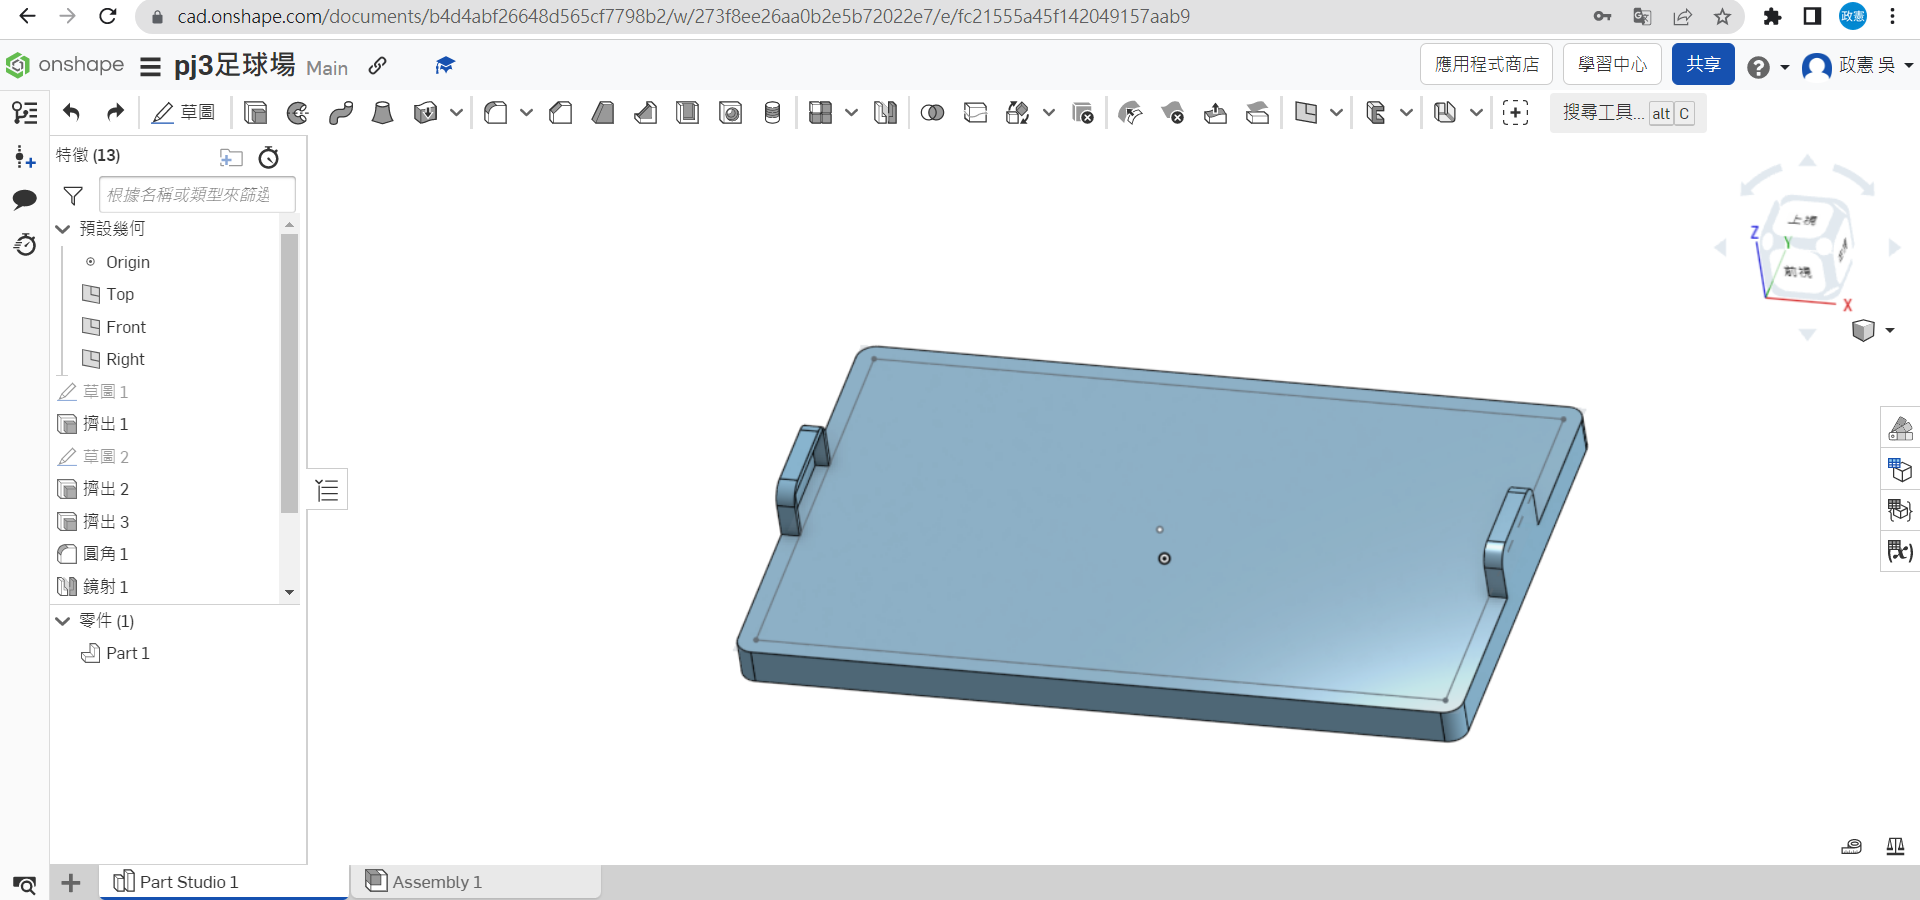
\includegraphics[width=8cm]{螢幕擷取畫面 2023-05-20 223657}
\caption{\Large 建立球場}\label{建立球場}
\end{center}
\end{figure}\

\newpage


\chapter{程式碼說明}
\renewcommand{\baselinestretch}{10.0} %設定行距
\pagenumbering{arabic} %設定頁號阿拉伯數字
\setcounter{page}{5}  %設定頁數
\fontsize{14pt}{2.5pt}\sectionef
\section{控制機器人程式}
\begin{figure}
\begin{center}
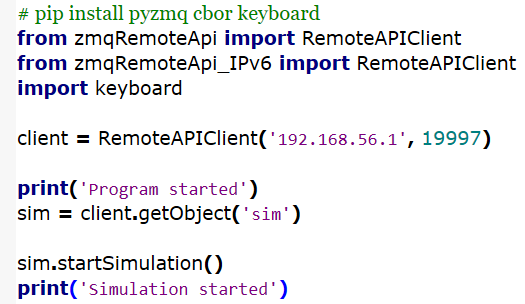
\includegraphics[height=8cm]{bubbleRob code 1}
\caption{\Large 控制機器人程式之一}\label{控制機器人程式之一}
\end{center}
\end{figure} 
使用 pip install pyzmq cbor keyboard 安裝了所需的套件,其中 pyzmq 是用於建立 ZeroMQ 連線,cbor 是用於將資料序列化和反序列化,keyboard 是用於操控鍵盤事件,使用 from zmqRemoteApi import RemoteAPIClient 和 from zmqRemoteApi_IPv6 import RemoteAPIClient 導入了用於建立與 CoppeliaSim 之間通訊的 Remote API 相關程式庫。這些程式庫提供了與 CoppeliaSim 的介面,使得可以通過程式碼控制仿真場景和物件,建立了一個 RemoteAPIClient 物件 client,並將 192.168.56.1 和 19997 分別作為 CoppeliaSim 的 IP 地址和連接埠進行初始化。這樣就建立了與 CoppeliaSim 的連線,使用 client.getObject('sim') 獲取了 CoppeliaSim 中的 sim 物件,該物件代表了整個仿真環境。透過這個物件,可以執行相關的仿真操作,再來透過  sim.startSimulation() 開始模擬。\\
\begin{figure}
\begin{center}
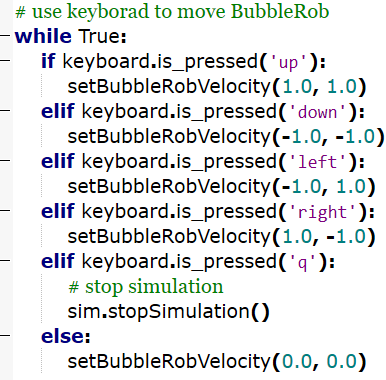
\includegraphics[height=8cm]{bubbleRob code 2}
\caption{\Large 控制機器人程式之二}\label{控制機器人程式之二}
\end{center}
\end{figure} 
這段程式碼是一個無窮迴圈,用於持續監聽鍵盤事件並根據按鍵的狀態來控制機器人的運動,如果按下 'up' 鍵,則呼叫 setBubbleRobVelocity(1.0, 1.0),將機器人的速度設定為正向。如果按下 'down' 鍵,則呼叫 setBubbleRobVelocity(-1.0, -1.0),將機器人的速度設定為反向。如果按下 'left' 鍵,則呼叫 setBubbleRobVelocity(-1.0, 1.0),將機器人的速度設定為左轉。如果按下 'right' 鍵,則呼叫 setBubbleRobVelocity(1.0, -1.0),將機器人的速度設定為右轉。如果按下 'q' 鍵,則停止仿真。若沒有按下上述任何按鍵,則呼叫 setBubbleRobVelocity(0.0, 0.0),將機器人的速度設定為零,即停止移動。
\section{模擬模型}

\newpage
\input{4_server.tex}
\input{5_training_result.tex}
\input{6_suggestion.tex}
\input{7_discussions.tex}
%=---------------------參考文獻----------------------=%
%\input{8_reference.tex}
%=---------------附錄-----------------=%
%\addcontentsline{toc}{chapter}{附錄} %新增目錄名稱
\input{9_appendix.tex}
\end{document}
